\documentclass[fleqn,10pt]{olplainarticle}
% Use option lineno for line numbers 

\title{Wormhole hack}
\author{Timotej Ponek}
\affil{timotej.ponek@gmail.com}

\keywords{Wormhole hack, Solana, Ethereum}

\begin{document}

\flushbottom
\maketitle
\thispagestyle{empty}

\section*{What is Wormhole}
Wormhole is a crosschain bridge that allows users to transfer their crypto assets from blockchain running under some protocol to another blockchain running under a different protocol. The mechanism of how it works can be described in these steps\cite{linkedIn}:
\begin{itemize}
  \item To move N tokens from blockchain A to blockchain B, the token owner first needs to lock N tokens into the bridge smart contract on blockchain A.
  \item After verification that N tokens have been locked, the bridge mints N equivalent tokens (or wrapped tokens) on blockchain B.
  \item To get back the original N tokens, the owner needs to burn N wrapped tokens on the bridge smart contract on blockchain B.
  \item After verification that N wrapped tokens have been burnt, the bridge will release N tokens on blockchain A and return them to the token owner.
\end{itemize}

Crosschain bridge could be likened to the old US gold certificates system. After depositing gold barse, the US bank issues gold certificates equivalent in value. The certificate is transferable and anyone can redeem it back to gold. The bank has to manage the security of gold storage and protect itself against counterfeit gold certificates.

Similar to the gold certificates system, crosschain bridges have two main security concerns:

\begin{itemize}
  \item Make sure tokens locked inside smart contract (gold bars) are safe
  \item Make sure minted wrapped tokens (gold certificates) are valid
\end{itemize}

\section*{What happened}
On 2nd February 2022, an attacker was able to exploit Wormhole protocol and gain wrapped Ethereum tokens (wETH) on Solana blockchain without depositing the equivalent amount of Ethereum to the bridge smart contract.

\section*{More details}
The root cause of the exploit was the usage of deprecated functions \cite{ackee, certik, immunebytes,linkedIn, rekt}, that allowed attacker to use a fake account for verification. The faulty code can be viewed \href{https://github.com/wormhole-foundation/wormhole/blob/ca509f2d73c0780e8516ffdfcaf90b38ab6db203/solana/bridge/program/src/api/verify_signature.rs#L68}{\color{red}here}.

\begin{listing}[H]

\begin{minted}[fontsize=\footnotesize,linenos,firstnumber=68]{rust}
pub fn verify_signatures(
  ctx: &ExecutionContext,
  accs: &mut VerifySignatures,
  data: VerifySignaturesData,
) -> Result<()> {
  accs.guardian_set
    .verify_derivation(ctx.program_id, &(&*accs).into())?;
  //...
\end{minted}
\begin{minted}[fontsize=\footnotesize,linenos,firstnumber=91, escapeinside=@@]{rust}
  //...
  let current_instruction = solana_program::sysvar::instructions::load_current_index( @\phantomsection\label{line:load_current_index}@
    &accs.instruction_acc.try_borrow_mut_data()?,
  );
  if current_instruction == 0 {
    return Err(InstructionAtWrongIndex.into());
  }

  // The previous ix must be a secp verification instruction
  let secp_ix_index = (current_instruction - 1) as u8;
  let secp_ix = solana_program::sysvar::instructions::load_instruction_at( @\phantomsection\label{line:load_instruction_at}@
    secp_ix_index as usize,
    &accs.instruction_acc.try_borrow_mut_data()?,
  )
  .map_err(|_| ProgramError::InvalidAccountData)?;
  //...
\end{minted}
%TODO pridať čo som sem zachytil a čo referencujem...
\caption{Usage of deprecated Solana functions in Wormhole code}
\label{list:code}

\end{listing}

In code snippet above, we can see that function \emph{verify\_signatures()} uses deprecated functions \emph{load\_current\_index()} (line \ref{line:load_current_index}) and \emph{load\_instruction\_at()} (line \ref{line:load_instruction_at}). Prior to the hack, the attacker must have found about the existance of these functions and their weaknesses, and figure out how they could be used to create the exploit.


A few hour before the hack happend, the attacker created an \href{https://etherscan.io/address/0x629e7da20197a5429d30da36e77d06cdf796b71a#internaltx}{\color{red}account on the Ethereum network} holding just $0.1$ ETH, that was later used in the exploit. To this account, he received 0.94 ETH from Tornado Cash, a privacy-focused Ethereum mixer, to facilitate the payment of transaction fees associated with their subsequent actions.

The exploit was condutected in following steps: At first, the attacker created a malicious account with fake instruction data. Then he invoked the \emph{verify\_signatures()} function with this forged account.

\begin{figure}[h!]
  \centering
  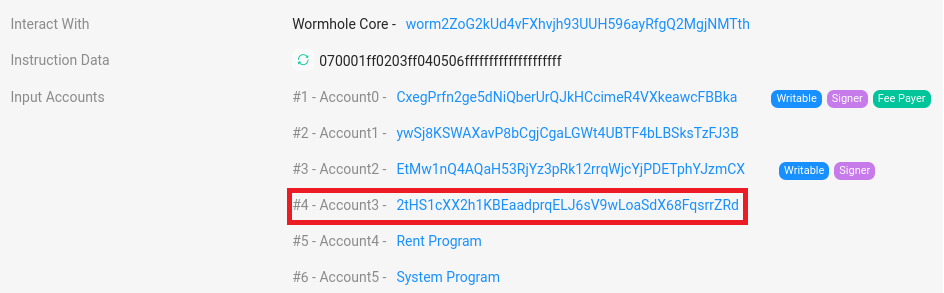
\includegraphics[width=\linewidth]{images/mal_acc.png}
  \caption{\href{https://solscan.io/tx/25Zu1L2Q9uk998d5GMnX43t9u9eVBKvbVtgHndkc2GmUFed8Pu73LGW6hiDsmGXHykKUTLkvUdh4yXPdL3Jo4wVS}{\color{blue}\emph{\underline{verify\_signatures}}} transaction with the malicious account (in red). If the account was valid, we would see string \emph{Sysvar: Instructions} in place of account address.}
  \label{fig:mal_acc}
\end{figure}

The \emph{verify\_signatures()} function loads the current instruction utilizing \emph{load\_current\_index()} (line \ref{line:load_current_index}) function. To attacker's advatage, this function does not validate whether the account at \emph{accs.instruction\_acc} (sysvar account) is actually a valid solana system sysvar account. So the attacker can insert any forged account with desired instruction because the account will never be checked for its validity.

We cannot say exactly what instruction the attacker inserted, but we can say for sure it was an instruction that allowed him to pass signature validation without ever invoking secp256k1 validation. He was able to return from the \emph{verify\_signatures()} function with a valid (but not verified by secp256k1) signature set account, and proceed further in \emph{post\_vaa()} function.

The \emph{post\_vaa()} function, not knowing it recieved unverified signatures, created the message account specifying the minting of 120,000 wETH (as the attacker desired) that was further passed to the \emph{complete\_wrapped()}.

\begin{figure}[h!]
  \centering
  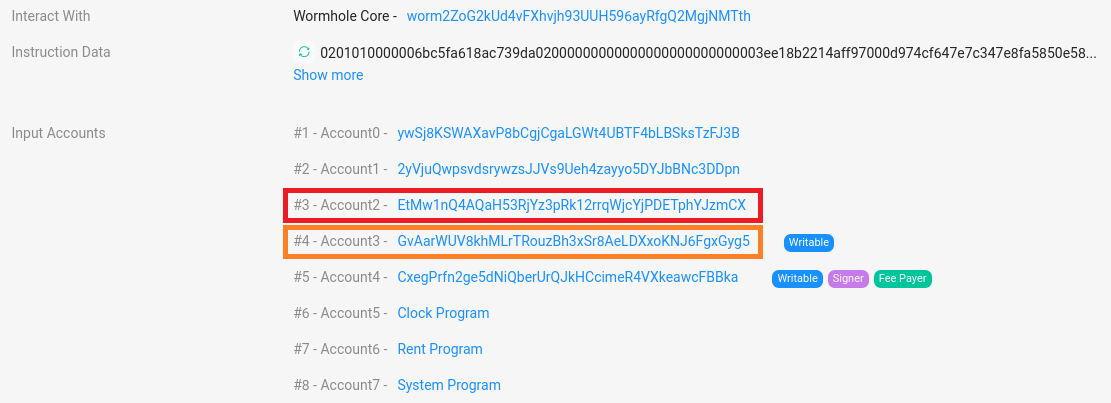
\includegraphics[width=\linewidth]{images/post_vaa.png}
  \caption{\href{https://solscan.io/tx/2SohoVoPDSdzgsGCgKQPByKQkLAXHrYmvtE7EEqwKi3qUBTGDDJ7DcfYS7YJC2f8xwKVVa6SFUpH5MZ5xcyn1BCK}{\color{blue}\emph{\underline{post\_vaa}}} transaction with unchecked but valid signatures (in red) and message account (in orange), stating $120,000$ wETH to be minted}
  \label{fig:post_vaa}
\end{figure}


In \emph{complete\_wrapped()} function, $120,000$ wETH tokens were minted and assigned to the attacker's account.

\begin{figure}[h!]
  \centering
  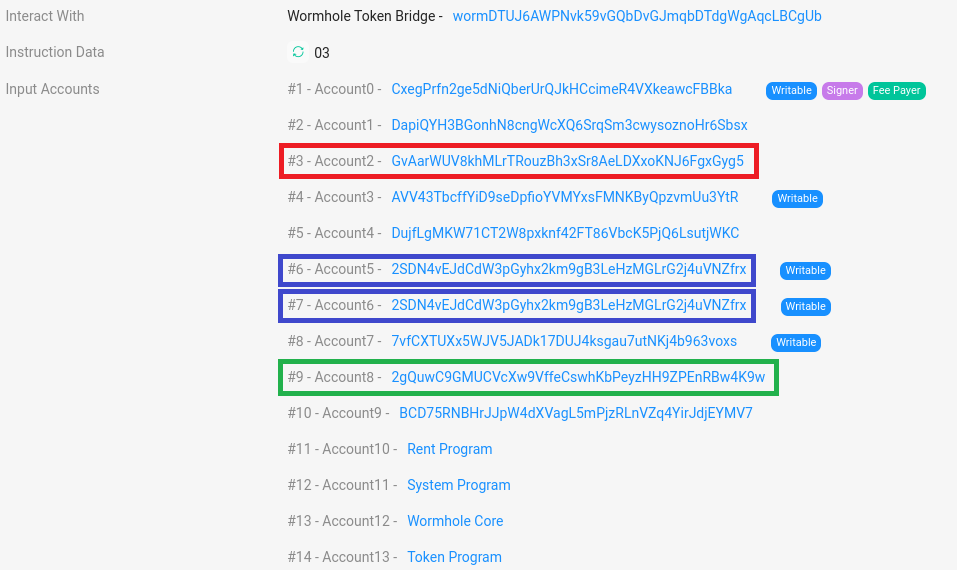
\includegraphics[width=\linewidth]{images/complete_wrapped.png}
  \caption{\href{https://solscan.io/tx/2zCz2GgSoSS68eNJENWrYB48dMM1zmH8SZkgYneVDv2G4gRsVfwu5rNXtK5BKFxn7fSqX9BvrBc1rdPAeBEcD6Es}{\color{blue}\emph{\underline{complete\_wrapped}}} transaction with malevolent message account (in red). In blue is account that will recieve the newly minted wETH (which is owned by the signer of the transaction) and in green is the mint authority (that only mints wETH relying that the checks were performed before)}
  \label{fig:complete_wrapped}
\end{figure}

\section*{Aftermath}

Following the minting of wETH, the attacker orchestrated a series of assets movements:
\begin{itemize}
  \item $93,750$ ETH was bridged back to Ethereum within 3 transactions, and still remains  in the hacker's wallet
  \item Remaining wETH was exchanged for $432,662.14$ SOL and $1444.16$ \$
\end{itemize}

Within the day the attack happend, Wormhole team sent to the attacker's Ethereum wallet a transaction  with a message offering him a whitehat agreement and 10 milion \$, if he returns the minted wETH and shares exploit details. Attacker did not respond.

On 3nd February 2022, the stolen assets were \href{https://twitter.com/jump_/status/1489301013408497666?}{replaced by the Wormhole's parent company Jump Crypto}, as the company believes in future of this project and wanted to maintain the trust in the project. The deprecated functions were also replaced with their checked versions, removing possibility of anyone using the same exploit again.

\bibliography{sample}

\end{document}